% This example is meant to be compiled with lualatex or xelatex
% The theme itself also supports pdflatex
\PassOptionsToPackage{unicode}{hyperref}
\documentclass[aspectratio=1610, 9pt]{beamer}

% Load packages you need here
\usepackage{polyglossia}
\setmainlanguage{german}

\usepackage{csquotes}


\usepackage{amsmath}
\usepackage{amssymb}
\usepackage{mathtools}

\usepackage{hyperref}
\usepackage{bookmark}

\usepackage{algorithm2e}
\usepackage{braket}

% load the theme after all packages

\usetheme[
  showtotalframes, % show total number of frames in the footline
]{tudo}

% Put settings here, like
\unimathsetup{
  math-style=ISO,
  bold-style=ISO,
  nabla=upright,
  partial=upright,
  mathrm=sym,
}

\title{Ist das Universum ein Computer?}
\author[J.~Speer]{Jannis Speer}
\date{17.12.20}
\institute{Big Questions Seminar}
\titlegraphic{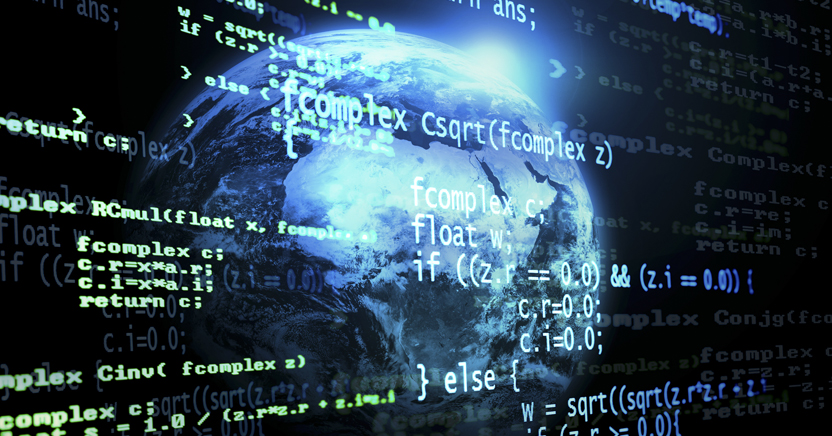
\includegraphics[width=0.7\textwidth]{images/titel.jpg}}


\begin{document}

\maketitle

\begin{frame}{Inhalt}
  \begin{itemize}
    \item Historische Einführung
    \item Information
    \item Turingmaschine
    \item Das Universum als universeller digitaler Computer
    \item Quantencomputer
    \item Das Universum als Quantencomputer
    \item Gegenposition - Das Universum ist kein Computer
  \end{itemize}
\end{frame}

%\begin{frame}{Inhalt}
%  \tableofcontents
%\end{frame}

\begin{frame}{Historische Einführung: Digitale Physik \footnote[1]{Digital physics, Wikipedia}}
  \begin{itemize}
    \item ursprüngliche Idee: Konrad Zuses Buch Rechnender Raum (1969)
    \item Hypothese: Universum ist digitaler Computer, genauer: zellulärer Automat
    \item Kompatibilität von Computern mit: \\Informationstheorie, statistischer Mechanik, Quantenmechanik
    \item Begriff geprägt durch  Edward Fredkin, alternativ: digitale Philosophie
    \item[]
    \item[\rightarrow] Digitale Physik: Theorien mit Prämisse, Universum durch Information beschreibbar ist
  \end{itemize}
\end{frame}

\begin{frame}{Digitale Physik - verschiedene Perspektiven \footnote[1]{Digital physics, Wikipedia}}
  \begin{itemize}
    \item Weizsäckers Quantentheorie der Ur-Alternativen:
      \begin{itemize}
        \item[\bullet] lediglich 2  Entitäten: Struktur der Zeit, binäre Alternativen
        \item[\bullet] abstrakt, nicht-lokal, keine feldtheoretischen Voraussetzungen
      \end{itemize}
    \item[]
    \item Wheelers It from Bit:
      \begin{itemize}
        \item[\bullet] klassisch: Realität existiert und wird gemessen
        \item[\bullet] hier: Messung schafft Realität
      \end{itemize}
    \item[]
    \item Pancomputationalism:
      \begin{itemize}
        \item[\bullet] Digitaler Computer vs. Quantencomputer
        \item[\bullet] Zufälligkeit und Komplexität des Universums? Effizienz?
      \end{itemize}
    \item[]
    \item Tegmarks Mathematical-Universe-Hypothese (MUH)
      \begin{itemize}
        \item[\bullet] Universum ist Mathematik, mathematische Existenz = physikalische Existenz
      \end{itemize}
  \end{itemize}
\end{frame}

\begin{frame}{Informationstheorie \footnote[3]{Information, Wikipedia} \footnote[4]{Information theory, Wikipedia}}
  \begin{figure}
    \begin{minipage}{0.7\textwidth}
      \begin{itemize}
        \item[] ... beschäftigt sich mit Quantifizierung, Speicherung und Übertragung von Information
        \item[]
        \item Konzept von Information hat verschiedene Bedeutungen \\verwandt mit: Nachricht, Kommunikation, Daten, Wissen
        \item hier: Information ist Folge von Symbolen aus einem Alphabet $Z = \{z_1, z_2,...,z_m\}$
        \item Informationsgehalt eines Zeichens: $I(z) = -\log_a(p_z)$ \\mit Wahrscheinlichkeit $p_z$, Mächtigkeit $a$
        \item Entropie eines Zeichens (Shannon): $H = E[I] = \sum_{z \in Z}{p_z I(z)} = - \sum_{z \in Z}{ p_z \log_a(p_z)}$
      \end{itemize}
    \end{minipage}
    \hfill
    \begin{minipage}{0.28\textwidth}
      \begin{figure}
        \includegraphics[width=0.8\textwidth]{images/binär.jpg}
        \caption{binäre Information. \footnotemark[2]}
      \end{figure}
    \end{minipage}
  \end{figure}
  \footnotetext[2]{cleanpng.com}
\end{frame}

\begin{frame}{physikalische Information und Entropie \footnote[5]{Physical information, Wikipedia}}
  \begin{itemize}
    \item Information beschreibt physikalisches System:
    \begin{itemize}
      \item[\bullet] Information löst Ungewissheit über Zustand eines physikalischen Systems
      \item[\bullet] Information ist Messung für Wahrscheinlichkeit eines Zustandes
    \end{itemize}
    \item[]
    \item $\text{fehlende Information} = \text{nötige Information, um Zustand zu beschreiben} = I = -k \sum_{i=1}^n{p_i \ln(p_i)}$ \\ mit $p_i$ der Wahrscheinlichkeiten der $n$ Zustände des Systems
    \item[]
    \begin{itemize}
      \item[\rightarrow] binäre Entropie der Informationstheorie: $k = \ln(2)^{-1}$
      \item[\rightarrow] Gibbs Entropie: $k = k_b$
    \end{itemize}
    \item Von Neumann Entropie, QM-Analogon: $S(\rho) = -Tr(\rho \ln\rho)$ mit Dichtematrix $\rho$
  \end{itemize}
\end{frame}

\begin{frame}{Algorithmische Informationstheorie \footnote[6]{Algorithmic information theory, Wikipedia}}
  \begin{itemize}
    \item Bestimmung des Informationsgehalt über Kolmogorow-Komplexität
    \item Kolmogorow-Komplexität:
    \begin{itemize}
      \item Informationsgehalts einer Zeichenkette = Länge des kleinsten Algorithmus, der Zeichenkette erzeugt
      \item nicht berechenbar, aufgrund des Halteproblems kleinster Algorithmus nicht bestimmbar
      \item unabhängig von der verwendeten universellen Programmiersprache abgesehen von additiver Konstante $c$
    \end{itemize}
  \end{itemize}
  \begin{figure}
    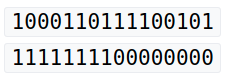
\includegraphics[width=0.2\textwidth]{images/kolmo.png}
    %\caption{binäre Information}
  \end{figure}
  \begin{itemize}
    \item algorithmic randomness:
    \begin{itemize}
      \item Zeichenkette ist zufällig, wenn Kolmogorow-Komplexität $>=$ Länge der Zeichenkette
      \item Zufälligkeit einer endlichen Zeichenkette abhängig von universellen Programmiersprache
      %\item Löf randomness: unendliche Folge $S$ ist $c$-inkompressibel, wenn Teilfolge $w$
    \end{itemize}
    \item algorithmic probability: kurze Algorithmen sind wahrscheinlicher als lange
  \end{itemize}
\end{frame}

\begin{frame}{Digitale Information, Boolesche Algebra, Klassische Logik}
  \begin{figure}
    \begin{minipage}{0.7\textwidth}
      \begin{itemize}
        \item Digitale Information: diskrete endliche Darstellung \rightarrow Ziffern, Buchstaben \rightarrow binär
        \item Boolesche Algebra mit Operatoren:
        \item[] $\land$ UND $\lor$ ODER $\lnot$ NICHT
        \item klassische Logik:
        \begin{itemize}
          \item Prinzip der Zweiwertigkeit
          \item Prinzip der Extensionalität
        \end{itemize}
      \end{itemize}
    \end{minipage}
    \hfill
    \begin{minipage}{0.28\textwidth}
      \begin{figure}
        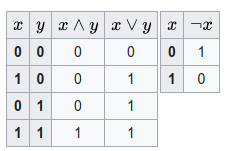
\includegraphics[width=0.8\textwidth]{images/bool.png}
        \caption{Boolesche Algebra. \footnotemark[7]}
      \end{figure}
    \end{minipage}
  \end{figure}
  \footnotetext[7]{Boolean Algebra}
\end{frame}

\begin{frame}{Vor Turing \footnote[8]{The Universe as Quantum Computer, Seth Lloyd, 2013}}
  \begin{itemize}
    \item Formulierung des Hilbertprogramms in 1920er
    \item Ziel: Nachweis der Widerspruchsfreiheit der Axiomensysteme der Mathematik
    \item[\rightarrow] Entscheidungsproblem: \enquote{First, was mathematics complete ... Second, was mathematics consistent ... \\ And thirdly, was mathematics decidable?}
    \item[\rightarrow] Beantwortung durch Gödels Unvollständigkeitssätze
    \item[]
    \item Was ist mathematisch exakt betrachtet ein Algorithmus?
  \end{itemize}

\end{frame}

\begin{frame}{Turingmaschine - informelle Einführung \footnote[8]{The Universe as Quantum Computer, Seth Lloyd, 2013}}
  \begin{figure}
    \begin{minipage}{0.49\textwidth}
      \begin{itemize}
        \item Interpretation von Logik als Prozess
        \item Definition Algorithmus und der Berechenbarkeit
        \item Analogie eines denkenden, lesenden und schreibenden Mathematikers
      \end{itemize}
      \begin{figure}
        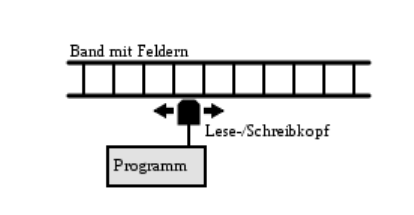
\includegraphics[width=0.8\textwidth]{images/turing.png}
        \caption{Turingmaschine. \footnotemark[9]}
      \end{figure}
    \end{minipage}
    \hfill
    \begin{minipage}{0.49\textwidth}
      \begin{itemize}
        \item Turingmaschine:
        \begin{itemize}
          \item Speicherband: unendlich viele, sequentiell angeordnete Felder
          \item Feld: nimmt einen von endlich vielen Zuständen an
          \item Lese-Schreib-Kopf: Verarbeitung von Information, nimmt einen von endlich vielen Zuständen an
        \end{itemize}
        \item Prozess:
        \begin{itemize}
          \item Kopf liest Zustand des aktuellen Feldes
          \item Kopf verarbeitet eignen Zustand und Feldzustand \\ (Überführungsfunktion)
          \item Änderung des Kopf und Feldzustandes
          \item Kopf bewegt sich ein Feld nach rechts oder links
        \end{itemize}
      \end{itemize}
    \end{minipage}
  \end{figure}
  \footnotetext[9]{Turingmaschine, Wikipedia}
\end{frame}

\begin{frame}{Anmerkungen zur Turingmaschine \footnote[8]{The Universe as Quantum Computer, Seth Lloyd, 2013}}
  \begin{figure}
    \begin{minipage}{0.29\textwidth}
      Algorithmus:
      \begin{itemize}
        \item Ausführbarkeit
        \item Statistische Finitheit
        \item Dynamische Finitheit
        \item Terminierung
        \item optional:
        \begin{itemize}
          \item[\bullet] Determiniertheit
          \item[\bullet] Determinismus
        \end{itemize}
      \end{itemize}
    \end{minipage}
    \hfill
    \begin{minipage}{0.69\textwidth}
      Universelle Turingmaschine (UTM):
      \begin{itemize}
        \item UTM simuliert beliebig Turingmaschine für beliebigen Input
        \item Speicherung der Turingmaschine und des Inputs auf Speicherband der UTM
        \item[\rightarrow] Halteproblem
      \end{itemize}
      \begin{figure}
        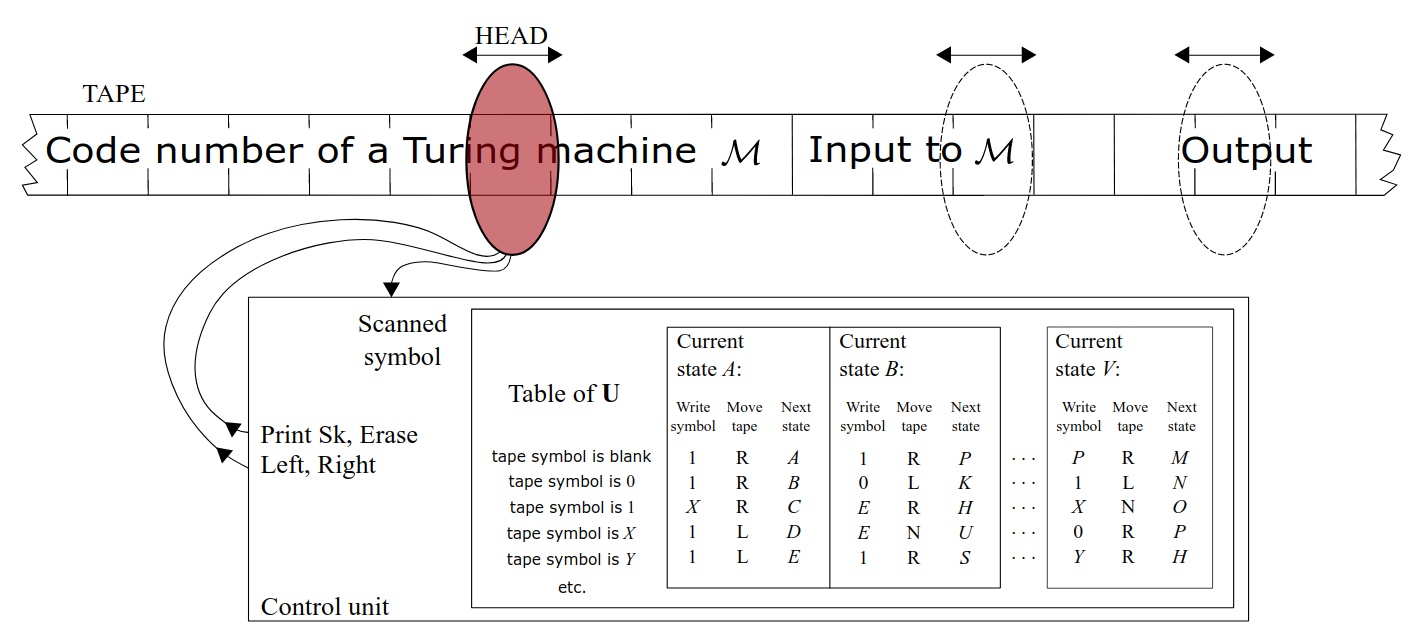
\includegraphics[width=0.75\textwidth]{images/UTM.png}
        \caption{Universelle Turingmaschine. \footnotemark[10]}
      \end{figure}
    \end{minipage}
  \end{figure}
  \footnotetext[10]{Universal Turing machine, Wikipedia}
\end{frame}

\begin{frame}{Anmerkungen zur Turingmaschine \footnote[8]{The Universe as Quantum Computer, Seth Lloyd, 2013}}
  \begin{figure}
    \begin{minipage}{0.55\textwidth}
      Halteproblem:
      \begin{itemize}
        \item Analog zu Gödels Unvollständigkeitssatz:
        \begin{itemize}
          \item Logik ist selbst-widersprechend und unvollständig
          \item Problem von auf sich selbst bezogene Behauptungen
          \item Lügner-Paradox: \enquote{Dieser Satz ist falsch.}
        \end{itemize}
        \item Keine UTM kann Frage beantworten, ob eine beliebige Turingmaschine anhält (Antwort liefert)
        \item Konstruktion von selbst-widersprechender UTM:
      \end{itemize}
      \begin{algorithm}[H]
        \KwResult{Hält beliebige Turingmaschine T an?}
        \Begin{
          T = beliebige Turingmaschine und I = beliebiger Input \;
            \While{T hat nicht angehalten == True}{Führe Schritt von T aus mit I\;}
          return Antwort \;
        }
      \end{algorithm}
    \end{minipage}
    \hfill
    \begin{minipage}{0.44\textwidth}
      Church-Turing-These:
      \begin{itemize}
        \item Jede intuitiv berechenbare Funktion kann durch eine UTM berechnet werden
        \item intuitiv berechenbar: mathematisch ungenauer Begriff
        \item Turing-berechenbar: Existenz von (terminierendem) Algorithmus
        \item[]
        \item striktere, physikalische Version: Church–Turing–Deutsch-Hypothese
        \item klassiche UTM kann jeden phyiskalischen Porzess simulieren
      \end{itemize}
    \end{minipage}
  \end{figure}
\end{frame}


\begin{frame}{Universum als universeller digitaler Computer \footnote[8]{The Universe as Quantum Computer, Seth Lloyd, 2013}}
  \begin{itemize}
    \item Digitaler Computer = System, das jede Folge von logischen Operationen ausführen kann
    \item Frage: Ist das Universum ein universeller digitaler Computer?
    \item[]
    \item[\rightarrow] Frage I: Kann das Universum universelle digitale Berchenungen nach Turing durchführen?
    \item[\rightarrow] Frage II: Keine eine klassische UTM effektiv die physikalischen Prozesse des Universum simulieren?
    \item[]
    \item naive Antwort: ja
    \item elektronischer Computer $\approx$ universeller digitaler Computer, der UTM simulieren kann
    \item Church–Turing–Deutsch-Hypothese
  \end{itemize}

\end{frame}

\begin{frame}{Universum als universeller digitaler Computer 2 \footnote[8]{The Universe as Quantum Computer, Seth Lloyd, 2013}}
  \begin{figure}
    \begin{minipage}{0.49\textwidth}
      Frage I:
      \begin{itemize}
        \item UTM benötigt unendlich viel Speicherplatz
        \item Liefer da Universum unendlich erweiterbaren Speicherplatz?
        \item echte elektrische Computer können als UTM verstanden werden, trotz endlichem Speicher
        \item Existenz von elektrischen Computer
        \item[\rightarrow] Antwort: Gesetze der Physik ermöglichen wahrscheinlich universellen digitalen Computer
      \end{itemize}
    \end{minipage}
    \hfill
    \begin{minipage}{0.49\textwidth}
      Frage II:
      \begin{itemize}
        \item UTM kann jeden berechenbaren physikalischen Prozess simulieren
        \item aber auch effizient auf kleinen Volumen von Raum und Zeit?
        \item[\rightarrow] Antwort: wahrscheinlich nicht
      \end{itemize}
    \end{minipage}
  \end{figure}
\end{frame}

\begin{frame}{Architektur des universellen digitalen Computers \footnote[8]{The Universe as Quantum Computer, Seth Lloyd, 2013}}
  \begin{figure}
    \begin{minipage}{0.49\textwidth}
      \begin{itemize}
        \item Gesetze der Physik sind: lokal, homogen und isotrop
        \item[\rightarrow] Computer-Version: zellulärer Automat
        \begin{itemize}
          \item Anordnung von Zellen mit endlichen Möglichkeit an Zusänden
          \item Zellen werden aktualisiert als Funktion des Zustandes der Zelle und ihrer Nachbarn
          \item Universum als sich selbst reproduzierender zellulärer Automat
          \item Universum besteht aus Bits, die lokalen logischen Operationen unterliegen
        \end{itemize}
        \item[]
        \item[\rightarrow] Frage III: Ist das Universum ein zellulärer Automat?
      \end{itemize}
    \end{minipage}
    \hfill
    \begin{minipage}{0.49\textwidth}
      \begin{figure}
        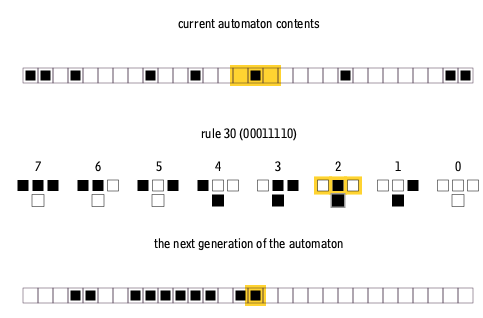
\includegraphics[width=0.8\textwidth]{images/zelle.png}
        \caption{eindimensionaler zellulärer Automat. \footnotemark[11]}
      \end{figure}
    \end{minipage}
    \footnotetext[11]{Cellular automaton, Wikipedia}
  \end{figure}


\end{frame}

\begin{frame}{Effizienz von digitalen Computern in Quantensimulationen \footnote[8]{The Universe as Quantum Computer, Seth Lloyd, 2013}}
  \begin{itemize}
    \item Bell Theorem:
    \item[] Quanteneffekte (Verschränkung) nicht berechenbar durch klassische lokale Modelle mit versteckten Variablen
    \item[]
    \item benötigen nicht-lokale Modelle mit:
    \begin{itemize}
      \item superluminare Kommunikation
      \item aufwendiger Simulation von Qubit
    \end{itemize}
    \item[\rightarrow] Antwort Frage III: Universum kein zellulärer Automat
    \item[]
    \item System mit $N$ Subssytemen, z.B. $N$ Kernspins, benötigt $O(2^N)$ klassische Bits
    \item benötigt exponentielle Kompression, die (noch) nicht existiert
    \item[\rightarrow] Antwort Frage II: klassicher digitalen Computern wahrscheinlich nicht effizient
  \end{itemize}
\end{frame}

\begin{frame}{Qubit \footnote[14]{Mit Quanten rechnen, Beatrice Marie Ellerhoff, Springer, 2020}}
  \begin{figure}
    \begin{minipage}{0.49\textwidth}
      \begin{itemize}
        \item Analogon zu klassischem Bit, Basis-Einheit der Quateninformation
        \item reiner Zustand eines Qubits als Superposition der zwei Basiszutände
        \item[] $\ket{\phi} = \alpha \ket{0} + \beta \ket{1} $ mit Basiszutänden $\ket{0} = \begin{pmatrix}1\\0\end{pmatrix}$, $\ket{1} = \begin{pmatrix}0\\1\end{pmatrix}$ und $|\alpha|^2 |\beta|^2 = 1$
        \item System aus mehreren Qubits mit Tensorprodukt:
        \item[] $\ket{0} \otimes \ket{0} = \ket{00} = \begin{pmatrix}1\\0\\0\\0\end{pmatrix}$, $\ket{01} = \begin{pmatrix}0\\1\\0\\0\end{pmatrix}$, $\ket{10} = \begin{pmatrix}0\\0\\1\\0\end{pmatrix}$, $\ket{11} = \begin{pmatrix}1\\0\\0\\1\end{pmatrix}$
        \item $n$-Qubits \rightarrow $2^n$-dim. Hilbertraum \rightarrow $2^n$ klassische Bits
      \end{itemize}
    \end{minipage}
    \hfill
    \begin{minipage}{0.49\textwidth}
      \begin{itemize}
        \item Bloch-Kugel - Repräsentation eines reinen Zustandes
        \item[] $\alpha = \exp(i\psi) \cdot \cos(\theta/2) = \cos(\theta/2)$
        \item[] $\alpha = \exp(i(\psi+\phi) \cdot \sin(\theta/2) = \exp(i\phi) \cdot \sin(\theta/2)$
        \begin{figure}
          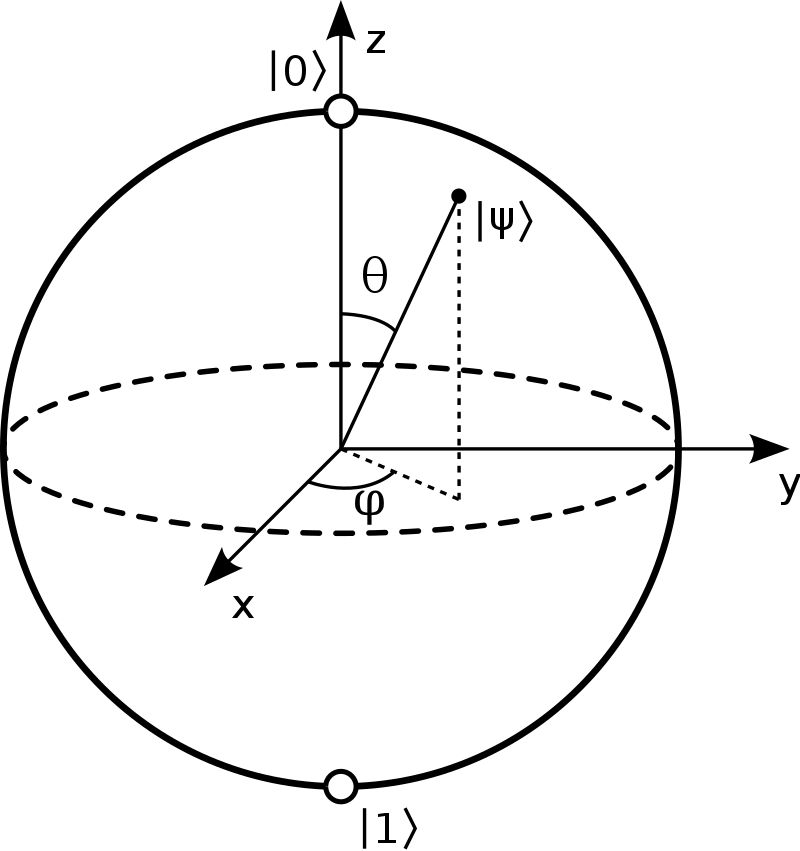
\includegraphics[width=0.56\textwidth]{images/Bloch.png}
          \caption{Bloch Kugel. \footnotemark[12]}
        \end{figure}
      \end{itemize}
    \end{minipage}
  \end{figure}
  \footnotetext[12]{Qubit, Wikipedia}
\end{frame}

\begin{frame}{Quantenverschränkung \footnote[14]{Mit Quanten rechnen, Beatrice Marie Ellerhoff, Springer, 2020} \footnote[12]{Qubit, Wikipedia} }
  \begin{figure}
    \begin{minipage}{0.49\textwidth}
      \begin{itemize}
        \item Produkt von 1-Qubit-Zuständen ergibt $n$-Qubit-Zustand:
        \item[] $\frac{1}{\sqrt{2}}(\ket{0}_1 + \ket{1}_1) \otimes \frac{1}{\sqrt{2}}(\ket{0}_2 - \ket{1}_2) = \frac{1}{2}(\ket{00}-\ket{01}+\ket{10}-\ket{11} ) $
        \item[]
        \item nicht jeder $n$-Qubit-Zustand darstellbar als Produkt von 1-Qubit-Zuständen \rightarrow Verschränkung
        \item einfachstes Beispiel: Bell-Zustand
        \item[] $\frac{1}{\sqrt{2}}(\ket{00} + \ket{11})$
      \end{itemize}
    \end{minipage}
    \hfill
    \begin{minipage}{0.49\textwidth}
      Im verschränkten Zustand:
      \begin{itemize}
        \item fehlende Information über Zustand des einzelnen Qubits
        \item[\rightarrow] gemischter Zustand, Beschreibung über Dichtematrix
        \item erst durch Messung ist genauer Zustand bekannt
        \item[]
        \item Messung des erste Qubits in perfekter Korrelation mit zweitem Qubit
        \item keine Abhängigkeit von Entfernung \rightarrow nichtlokal
      \end{itemize}
      %gemischter Zustand:
      %\begin{itemize}
      %  \item befindet sich in Bloch Kugel
      %  \item 3 Freiheitsgrade (zusätlich zu $\phi$ und $\theta$ noch $r$)
      %\end{itemize}
    \end{minipage}
  \end{figure}
\end{frame}

\begin{frame}{Quantencomputer}
  \begin{figure}
    \begin{minipage}{0.48\textwidth}
      \begin{itemize}
        \item wichtige Prinzipien: Superposition und Verschränkung
        \item Quantenregister \leftarrow \rightarrow klassische Register (Zeichenkette)
        \item Quantengatter \leftarrow \rightarrow Logikgatter
      \end{itemize}
    \end{minipage}
    \hfill
    \begin{minipage}{0.48\textwidth}
      \begin{figure}
        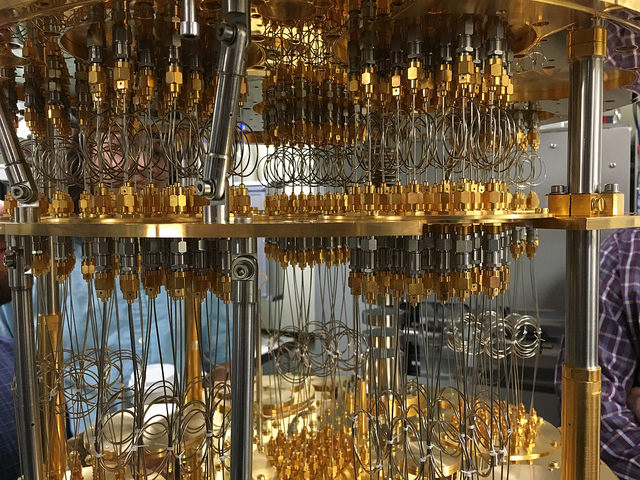
\includegraphics[width=0.9\textwidth]{images/Quantencomputer.jpg}
        \caption{IBM Quantencomputer. \footnotemark[15]}
      \end{figure}
    \end{minipage}
    \footnotetext[15]{IBM Quantencomputer, digitalbusiness-cloud.de, 2016}
  \end{figure}


\end{frame}

\begin{frame}{Quantenregister \footnote[13]{Quantencomputer, Wikipedia}}
  \begin{itemize}
    \item Analog zu klassischem Computer: Zusammenfassung mehrerer Bits zu Register (Zeichenkette)
    \item[\rightarrow] Quantenregister = Tensorprodukt einzelner 1-Qubit-Zustände
    \item Register im Zustand 01010100 \rightarrow Quantenregister  im Zustand $\ket{01010100}$
    \item Zustand eines Quantenregisters mit $N$-Qubits:
    \item[] $\psi = \sum_{i_1 ...i_N} c_{i_1 ...i_N} \ket{i_1 ... i_N} $
    \item[]
    \item Messung des Zustand des Quantenregisters \rightarrow Informationsgehalt: Quantenregister = klassisches Register
  \end{itemize}
\end{frame}

\begin{frame}{Quantengatter \footnote[14]{Mit Quanten rechnen, Beatrice Marie Ellerhoff, Springer, 2020}}
  \begin{itemize}
    \item Logikgatter: Anordnung zur Ausführung logischer Operatoren auf Bits
    \item Quantengatter: Ausführung von Operatoren auf Qubit-Zuständen
    \item $U \ket{\phi_1} = \ket{\phi_2}$
    \item[]
    \item Beispiele:
  \end{itemize}
  \begin{figure}
    \begin{minipage}{0.49\textwidth}
      \begin{figure}
          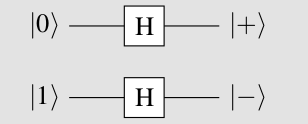
\includegraphics[width=0.56\textwidth]{images/Hadamard.png}
          \caption{Hadamard-Gatter. \footnotemark[14]}
      \end{figure}
      \begin{itemize}
        \item[] $\frac{1}{\sqrt{2}} (\ket{0} + \ket{1}) = \ket{+}$,  $\frac{1}{\sqrt{2}} (\ket{0} - \ket{1}) = \ket{-}$
      \end{itemize}
    \end{minipage}
    \hfill
    \begin{minipage}{0.49\textwidth}
      \begin{figure}
          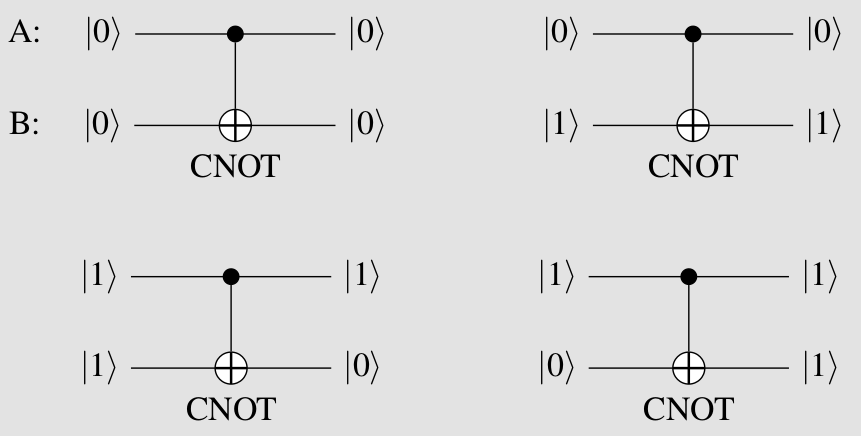
\includegraphics[width=0.8\textwidth]{images/CNOT.png}
          \caption{CNOT-Gatter. \footnotemark[14]}
      \end{figure}
    \end{minipage}
  \end{figure}
\end{frame}

\begin{frame}{Kombination von Hadamard und CNOT für Bell-Zustand}
  \begin{figure}
      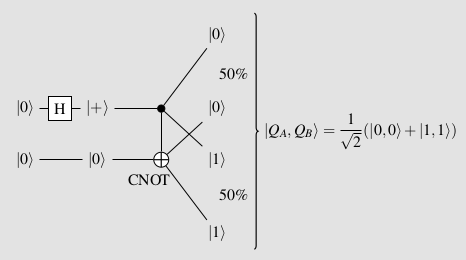
\includegraphics[width=0.7\textwidth]{images/kombi.png}
      \caption{kombiniertes Hadamard- und CNOT-Gatter für Bell-Zustand. \footnote[14]{Mit Quanten rechnen, Beatrice Marie Ellerhoff, Springer, 2020}}
  \end{figure}
\end{frame}

\begin{frame}{Universum als Quantencomputer \footnote[8]{The Universe as Quantum Computer, Seth Lloyd, 2013}}
  \begin{itemize}
    \item Frage I: Erlaubt das Universum Quantencomputer?
    \item Antwort: ja, aber...
    \begin{itemize}
      \item[] ... Unbegrenzter Speicherplatz im Universum?
      \item[] ... Technische Fähigkeit, großangelegten Quantencomputer zu bauen fehlt uns (noch)
    \end{itemize}
    \item[]
    \item Frage II: Kann ein Quantencomputer effektiv die physikalischen Prozesse des Universum simulieren?
    \item Antwort: wahrscheinlich
    \begin{itemize}
      \item[] Prinzipien des Universums = Prinzipien von Quantencomputern
      \item[] Grenze für Hochenergie-Dynamik \rightarrow Planck-Skala
    \end{itemize}
    \item[]
    \item Frage III: Ist das Universum ein quantenphysikalischer zellulärer Automat?
    \item Antwort: wahrscheinlich
    \begin{itemize}
      \item[] Ableitung von zellulärem Automat aus Gitter-Eichtheorien
      \item[] aktuelle Beobachtungen: Prozesse des Universums sind homogen, isotrop und lokal
    \end{itemize}
  \end{itemize}

\end{frame}

\begin{frame}{Universum als quantenphysikalischer zellulärer Automat \footnote[8]{The Universe as Quantum Computer, Seth Lloyd, 2013}}
  \begin{itemize}
    \item Antwort auf Frage:
    \item Warum ist das Universum so strukturiert und trotzdem so komplex?
    \item[]
    \item Erwartung: einfacher Anfangszustand + einfache Gesetze \rightarrow einfacher aktueller Zustand
    \item Realität: Universum voller komplexer Strukturen
    \item[]
    \item Erklärung:
    \begin{itemize}
      \item bildliche Vorstellung: Affen bedienen Tastatur des Universums
      \item produzieren viele \underline{nicht} funktionierende Programme
      \item aber auch \underline{zufällig} viele funktionierende \underline{kurze} Programme
      \item kurze Programme erzeugen scheinbar komplexe Strukturen \rightarrow Kolmogorow-Komplexität vs. klassicher Informationsgehalt
      \item \underline{kürzesten} Programme sind \underline{zufällig}, sonst existieren noch kürzere Programme, die selbe Struktur erzeugen
      \item[\rightarrow] Quantenfluktuation für Erzeugung von zufälligen Bits
    \end{itemize}
  \end{itemize}

\end{frame}

\begin{frame}{Kritikpunkte: Universum als Quantencomputer \footnote[16]{The Computational Universe, Jürgen Schmidhuber, 2006}}
  \begin{itemize}
    \item Fragen nicht geklärt:
    \item[] Ist das Universum deterministisch oder zufällig?
    \item[] Was ist Effizienz von klassischen Computern für Quanteneffekte?
    \item[]
    \item echter Zufall = maximale Kolmogorow-Komplexität
    \item Prinzip von Occam's razor: Favorisiere einfache Erklärungen \rightarrow Echter Zufall ist keine gute Wahl
    \item[]
    \item Annahme: \underline{kürzesten} Programme sind \underline{zufällig}, sonst existieren noch kürzere Programme, die selbe Struktur erzeugen
    \item nicht belegbar \rightarrow Kolmogorow-Komplexität/Halteproblem nicht berechenbar
  \end{itemize}

\end{frame}

\begin{frame}{Gegenposition - Das Universum ist kein Computer \footnote[17]{Questioning the Foundations of Physics, Anthony Aguirre, Brendan Foster and Zeeya Merali, Springer, 2014}}
  \begin{itemize}
    \item Newtonian Schema Universe (NSU):
    \begin{itemize}
      \item Universum beschrieben durch dynamische Gleichungen
      \item Universum als Computer: Anfangszustand $\quad \begin{matrix*}\text{Berechnung}\\ \longrightarrow\end{matrix*} \quad $ Endzustand
    \end{itemize}
    \item[]
    \item Lagrangian Schema Universe (LSU):
    \begin{itemize}
      \item Universum beschrieben durch Lagrangedichte
      \item Universum als globales vierdimensionales Randwertproblem
      \item[]
      \item Vorteile:
      \item gleicher Lösungsweg für jede Teilmenge des Universum \rightarrow Änlichkeit von kausal nicht verbundenen Teile des Universums
      \item elegante Einbindung von Quanteneffekten und Allgemeine Relativitätstheorie \rightarrow keine Trennung von Raum und Zeit wie bei dynamischer Berechnung von Computer
    \end{itemize}
  \end{itemize}

\end{frame}

\begin{frame}{Ausblick}
  \begin{itemize}
    \item Ist das Universum ein digitaler Computer?
    \item dafür sprechen:
    \begin{itemize}
      \item enger Zusammenhang zwischen Informationsverarbeitung zwischen Computern und dem Universum
      \item Effizienz von digitalen Computern fraglich
    \end{itemize}
    \item[]
    \item Ist das Universum ein Quantencomputer?
    \begin{itemize}
      \item Quantencomputer kann fundamentalen Quanteneffekte des Universums beschrieben
      \item Erklärung für Koexistenz von Zufälligkeit und Ordnung des Universums
    \end{itemize}
    \item[]
    \item offene Fragen:
    \begin{itemize}
      \item Ist das Universum deterministisch oder zufällig?
      \item Bietet das Universum unendlich viel Speicherplatz?
      \item Wie viel Information beinhaltet das Universum? \rightarrow nächster Vortrag
    \end{itemize}
  \end{itemize}
\end{frame}

\begin{frame}{Literaturverzeichnis}
  \begin{itemize}
    \item[1] https://en.wikipedia.org/wiki/Digital\_physics
    \item[2] https://de.cleanpng.com/png-5mw0s2/
    \item[3] https://en.wikipedia.org/wiki/Information
    \item[4] https://en.wikipedia.org/wiki/Information\_theory
    \item[5] https://en.wikipedia.org/wiki/Physical\_information
    \item[6] https://en.wikipedia.org/wiki/Algorithmic\_information\_theory
    \item[8]
    \item[7] https://en.wikipedia.org/wiki/Boolean\_algebra
    \item[9] https://de.wikipedia.org/wiki/Turingmaschine
    \item[10] https://en.wikipedia.org/wiki/Universal\_Turing\_machine
    \item[11] https://en.wikipedia.org/wiki/Cellular\_automaton
    \item[12] https://en.wikipedia.org/wiki/Qubit
    \item[13] https://de.wikipedia.org/wiki/Quantencomputer
    \item[14]
    \item[15] https://www.digitalbusiness-cloud.de/ibm-quantencomputer-ueber-die-cloud-fuer-jedermann/
    \item[16]
    \item[17]
  \end{itemize}

\end{frame}

\end{document}
